\chapter{Architettura del Prodotto}\label{ArchitetturaDelProdotto}
L'architettura generale del software$_{\scaleto{G}{3pt}}$ \textit{Gathering-Detection-Platform} è un'architettura monolitica distribuita.
Si tratta di due file eseguibili, scritti in Python$_{\scaleto{G}{3pt}}$, che sono rispettivamente il modulo Acquisition e il modulo Prediction.
Il primo viene utilizzato per acquisire le informazione estrapolate dalle live webcams delle città, il secondo invece viene utilizzato per calcolare predizioni su periodi di tempo futuri, utilizzando il machine-learning$_{\scaleto{G}{3pt}}$.
Entrambi sono collegati ad un database, il quale serve per archiviare ed esportare i dati in esso.
Il terzo, ed ultimo, modulo riguarda la web-app$_{\scaleto{G}{3pt}}$ vera e propria, che permette all'utente utilizzatore di visualizzare la heat-map$_{\scaleto{G}{3pt}}$ relativa alla città.
La web-app$_{\scaleto{G}{3pt}}$ è composta da due sotto-moduli definiti rispettivamente back-end$_{\scaleto{G}{3pt}}$ e front-end$_{\scaleto{G}{3pt}}$, all'interno del primo è presente l'applicazione di Spring, la quale imposta un server per eseguire i servizi per il front end, mentre la seconda è la parte dell'applicazione che mostra i dati all'utente finale. Il back-end$_{\scaleto{G}{3pt}}$ e front-end$_{\scaleto{G}{3pt}}$ dialogano attraverso richieste di tipo HTTP, il back-end$_{\scaleto{G}{3pt}}$ mette a disposizione un server$_{\scaleto{G}{3pt}}$ con servizi di tipo REST che effettuano solo query al database di tipo GET. Il front-end$_{\scaleto{G}{3pt}}$ una volta ottenuta l'informazione modifica attraverso metodi javascript$_{\scaleto{G}{3pt}}$ la mappa che l'utente visualizza insieme alle sue componenti.
Nella sezione successiva vengono inseriti i diagrammi di ogni modulo descritto, questo permette di avere una visione globale di ogni modulo nelle sue dipendenze a librerie esterne, nelle sue attività che svolgono e nelle sue componenti. Questi diagrammi sono stati scritti seguendo i principi UML.

\section{Architettura modulo Acquisition}\label{ArchitetturaDelProdottoArchitetturaModuloAcquisition}
\subsection{Diagramma dei Package}\label{ArchitetturaDelProdottoArchitetturaModuloAcquisitionDiagrammaDeiPackage}
Il modulo Acquisition utilizza due librerie esterne a Python$_{\scaleto{G}{3pt}}$, la prima è la libreria di Kafka$_{\scaleto{G}{3pt}}$ per creare applicativi di tipo consumer e producer e la seconda è MongoEngine$_{\scaleto{G}{3pt}}$ per creare una connessione ad un database di MongoDB$_{\scaleto{G}{3pt}}$.
\begin{figure}[H]
  \begin{center}
    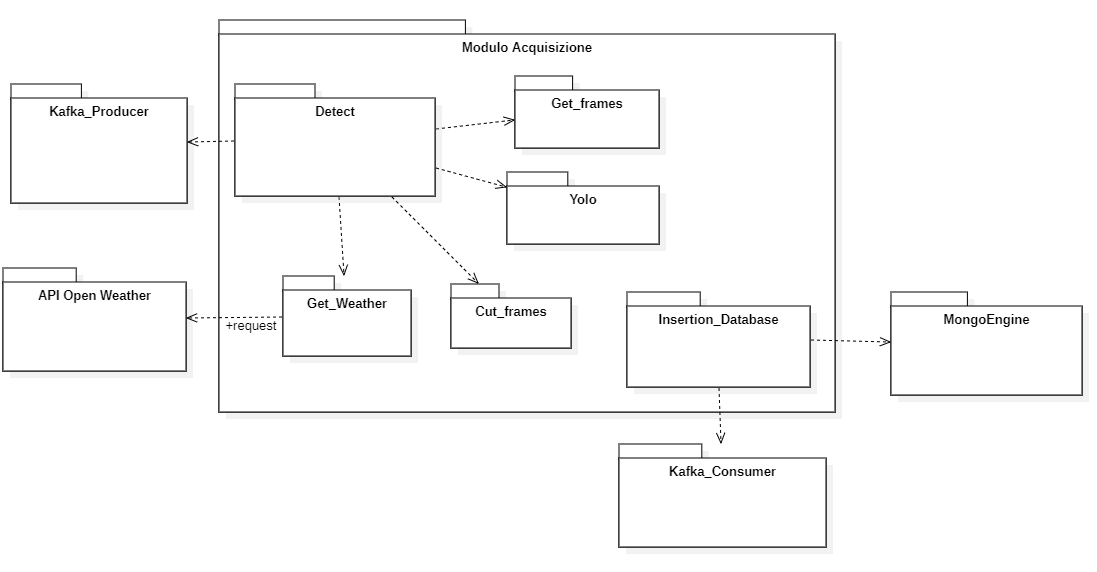
\includegraphics[scale=0.6]{../immagini/diag_PB/diag_pack_acqui.png}
    \caption{Diagramma dei package del modulo Acquisition}
  \end{center}
\end{figure}

\subsection{Diagrammi di attività}\label{ArchitetturaDelProdottoArchitetturaModuloAcquisitionDiagrammiDIAttività}
Di seguito vengono descritte le attività più importanti svolte nel modulo Acquisition.
\begin{figure}[H]
  \begin{center}
    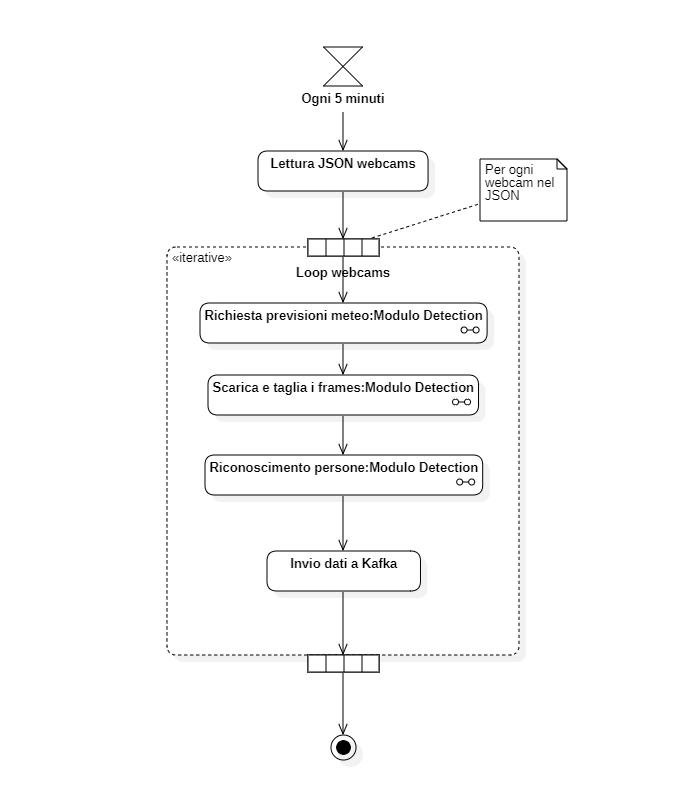
\includegraphics[scale=0.8]{../immagini/diag_PB/detection.png}
    \caption{Diagramma di attività dell'eseguibile Detection}
  \end{center}
\end{figure}


Da questo diagramma si può notare come il ciclo venga ripetuto ogni 5 minuti e per ogni webcam presente all'interno del file JSON associato.
Il lasso di tempo pari a 5 minuti è stato deciso arbitrariamente dopo aver testato la velocità di riconoscimento persone effettuato da YOLO v3.
È stato riscontrato che per elaborare 6 frame vengono impiegati circa 2 secondi per ciascuno.
Successivamente vengono illustrate tutte le sotto-attività completate durante il ciclo di operazioni dell'attività principale di acquisizione.
\begin{figure}[H]
  \begin{center}
    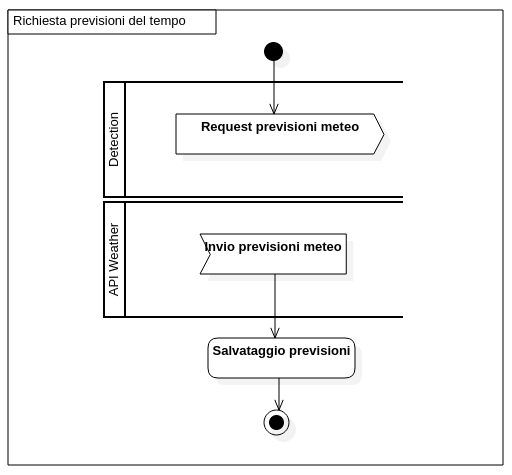
\includegraphics[scale=0.8]{../immagini/diag_PB/previsioni_del_tempo.png}
    \caption{Diagramma di sotto-attività dell'acquisizione delle previsioni meteo}
  \end{center}
\end{figure}
Nel diagramma in figura 5.3 viene illustrata la richiesta di informazioni all'API per le condizioni meteo in cui è posizionata la webcam. Il programma rimane in attesa della risposta dall'API, che alla sua ricezione completa l'attività salvando i dati forniti in una variabile.
\begin{figure}[H]
  \begin{center}
    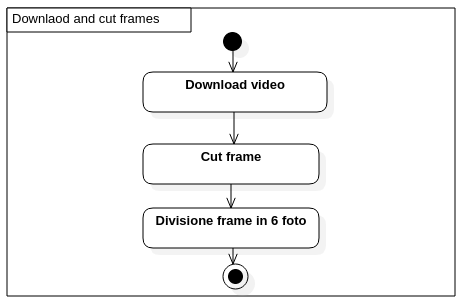
\includegraphics[scale=0.65]{../immagini/diag_PB/download_e_cut_frames.png}
    \caption{Diagramma di sotto-attività di download e taglio frame}
  \end{center}
\end{figure}
Nel diagramma in figura 5.4 vengono illustrate l'ordine di esecuzione delle attività di download del video, viene estrapolato un'immagine dal video e dividere l'immagine in 6 frame.
\begin{figure}[H]
  \begin{center}
    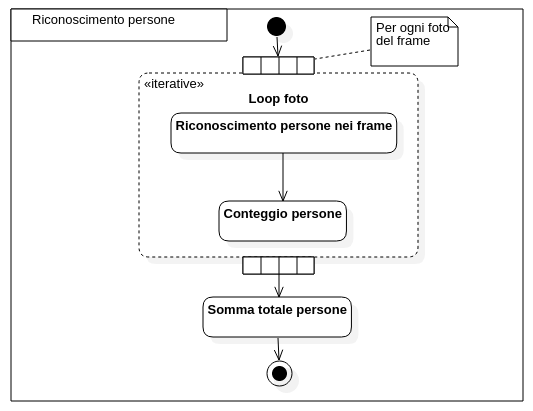
\includegraphics[scale=0.7]{../immagini/diag_PB/conta_persone.png}
    \caption{Diagramma di sotto-attività del conta persone}
  \end{center}
\end{figure}
Nel diagramma in figura 5.5 vengono mostrate le operazioni ripetute all'interno di ogni frame$_{\scaleto{G}{3pt}}$ per ottenere il numero di persone in ognuno di essi. Completate queste operazioni iterative ogni conteggio viene sommato per trovare il totale delle persone presenti nell'immagine intera.
\begin{figure}[H]
  \begin{center}
    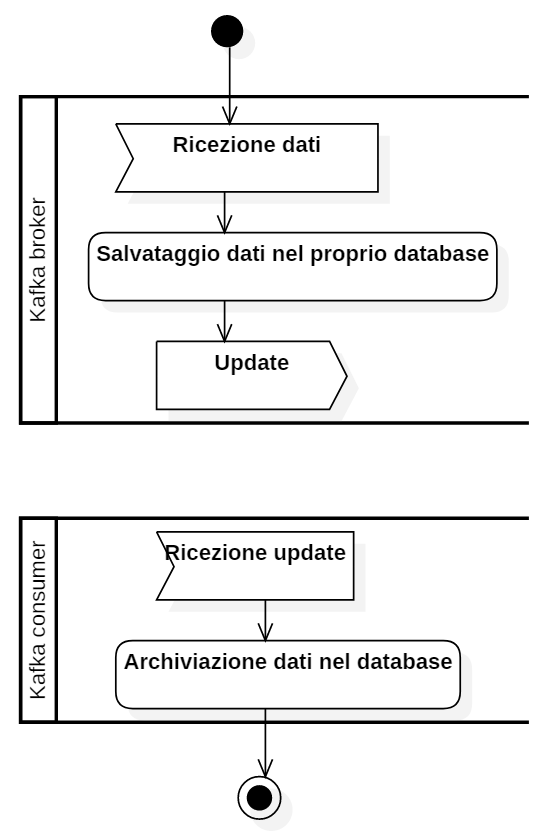
\includegraphics[scale=0.4]{../immagini/diag_PB/kafka.png}
    \caption{Diagramma di attività di Kafka}
  \end{center}
\end{figure}
Nel diagramma in figura 5.6 viene illustrato il funzionamento interno di Apache Kafka$_{\scaleto{G}{3pt}}$, il quale invia le informazioni al programma che consuma i dati inserendoli all'interno del database$_{\scaleto{G}{3pt}}$.

\section{Architettura modulo Prediction}\label{ArchitetturaDelProdottoArchitetturaModuloPrediction}
\subsection{Diagramma dei package}\label{ArchitetturaDelProdottoArchitetturaModuloPredictionDiagrammaDeiPackage}
Nel modulo Prediction vengono utilizzate le librerie esterne Pandas$_{\scaleto{G}{3pt}}$, MongoEngine$_{\scaleto{G}{3pt}}$ e Scikit-Learn$_{\scaleto{G}{3pt}}$ (abbreviato in Sklearn nella libreria). La libreria più importante è Scikit-Learn$_{\scaleto{G}{3pt}}$ della quale utilizziamo i metodi per il Preprocessing dei dati, la creazione di modelli con Model\_selection e il tipo di modello per generare le predizioni, il Random Forest Regression.
\begin{figure}[H]
  \begin{center}
    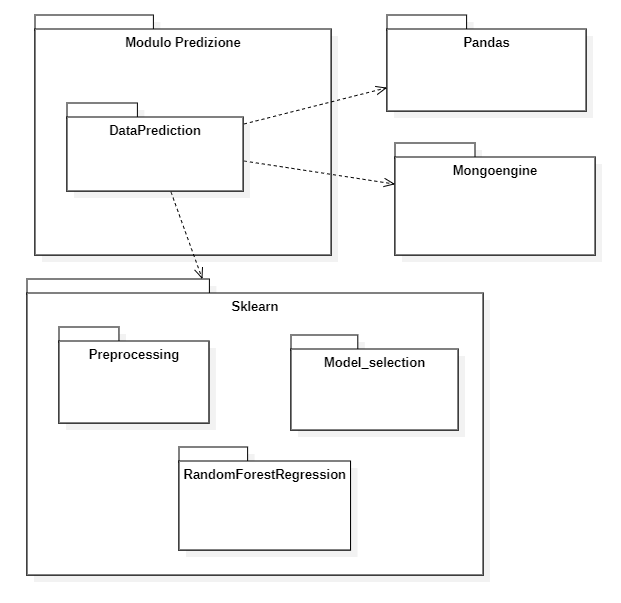
\includegraphics[scale=0.8]{../immagini/diag_PB/diag_pack_pred.png}
    \caption{Diagramma dei package del modulo Prediction}
  \end{center}
\end{figure}

\subsection{Diagramma di attività}\label{ArchitetturaDelProdottoArchitetturaModuloPredictionDiagrammaDiAttività}
Il diagramma dell'attività del modulo Prediction descrive le operazioni eseguite dal programma per generare le predizioni della zona presa in esame. Il programma legge dal file \textit{webcams.json} la lista di zone di cui bisogna effettuare le predizioni. Utilizzando le zone si prelevano i dati reali elaborati dal modulo Acquisition dal database, una volta ottenuti si controllano e vengono eliminati i dati ritenuti difettosi. Viene creato un dataset con i valori riferiti alle predizioni nel quale verranno inseriti i risultati del modello machine learning. Successivamente viene definito un modello utilizzando il tipo di regressione \textit{Random Forest Regression} e viene allenato con i valori prelevati dal database. Infine si utilizza il dataset creato precedentemente per ricavare le predizioni usando il modello allenato, a questo punto si archivia il dataset con i risultati del modello nel database.
\begin{figure}[H]
  \begin{center}
    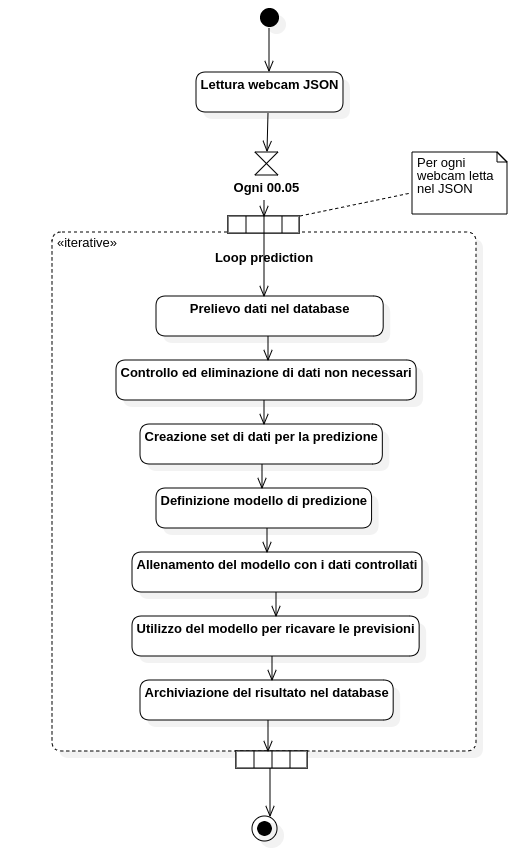
\includegraphics[scale=0.6]{../immagini/diag_PB/prediction_activity.png}
    \caption{Diagramma di attività dell'eseguibile DataPrediction}
  \end{center}
\end{figure}



\section{Architettura modulo Web-app}\label{ArchitetturaModuloWebApp}
Il modulo della web-app$_{\scaleto{G}{3pt}}$, come descritto in precedenza, è diviso in due sotto-moduli rispettivamente per il back-end$_{\scaleto{G}{3pt}}$ e front-end$_{\scaleto{G}{3pt}}$.
Il front-end è stato sviluppato seguendo le \textit{best practices} definite dalla documentazione di Vue.js e data la nostra poca conoscenza di questo linguaggio di programmmazione non è stato possibile definire un pattern strutturale per il modulo sviluppato.
L'archiviazione dei dati è stata sviluppata utilizzando un database non relazionale, il cui schema viene spiegato in seguito. Tutte le informazioni dei dati raccolti sono inserite all'interno di una collazione denominata Detection. Ogni dato è composto da 13 campi:
\begin{itemize}
	\item \textbf{\_id}: identifica univocamente il dato corrente;
	\item \textbf{id\_webcam}: individua l'id della webcam utilizzata per raccogliere il dato;
	\item \textbf{city}: individua la città in cui si trova la webcam;
	\item \textbf{location}: individua la locazione della webcam nella città;
	\item \textbf{latitude}: individua la latitudine della webcam;
	\item \textbf{longitude}: individua la longitudine della webcam;
	\item \textbf{numPeople}: individua il numero di persone presenti in quel momento;
	\item \textbf{date}: individua la data di raccolta del dato;
	\item \textbf{time}: individua l'orario di raccolta del dato;
	\item \textbf{type}: individua il tipo di dato se è 0 il dato è reale, se è 1 il dato è ricavato da una predizione;
	\item \textbf{weather\_description}: individua il tempo meteorologico;
	\item \textbf{temperature}: individua la temperatura;
	\item \textbf{day\_of\_week}: individua il giorno della settimana.
\end{itemize}
\subsection{Diagrammi dei package}\label{ArchitetturaModuloWebAppDiagrammiDeiPackage}
Di seguito vengono visualizzate le dipendenze dei due sotto-moduli, per il back-end$_{\scaleto{G}{3pt}}$ è solo necessaria la libreria del framework$_{\scaleto{G}{3pt}}$ Spring$_{\scaleto{G}{3pt}}$, mentre per il front-end$_{\scaleto{G}{3pt}}$ sono necessarie varie librerie per ogni componente della web-app$_{\scaleto{G}{3pt}}$.
\begin{figure}[H]
  \begin{center}
    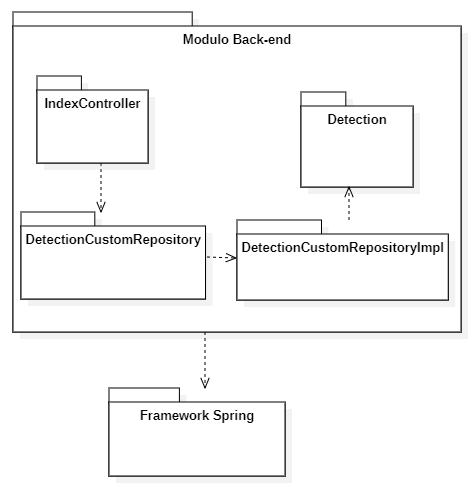
\includegraphics[scale=0.8]{../immagini/diag_PB/diag_pack_spring.png}
    \caption{Diagramma dei package di Spring}
  \end{center}
\end{figure}

\begin{figure}[H]
  \begin{center}
    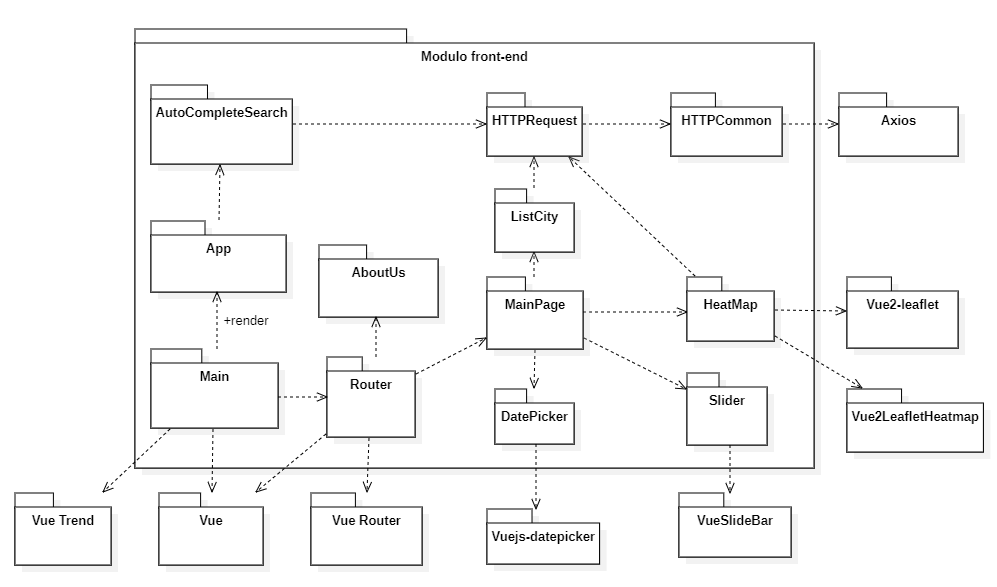
\includegraphics[scale=0.65]{../immagini/diag_PB/diag_pack_vue.png}
    \caption{Diagramma dei package del front-end in Vue}
  \end{center}
\end{figure}

\subsection{Diagrammi delle classi}\label{ArchitetturaModuloWebAppDiagrammiDelleClassi}
\begin{figure}[H]
  \begin{center}
    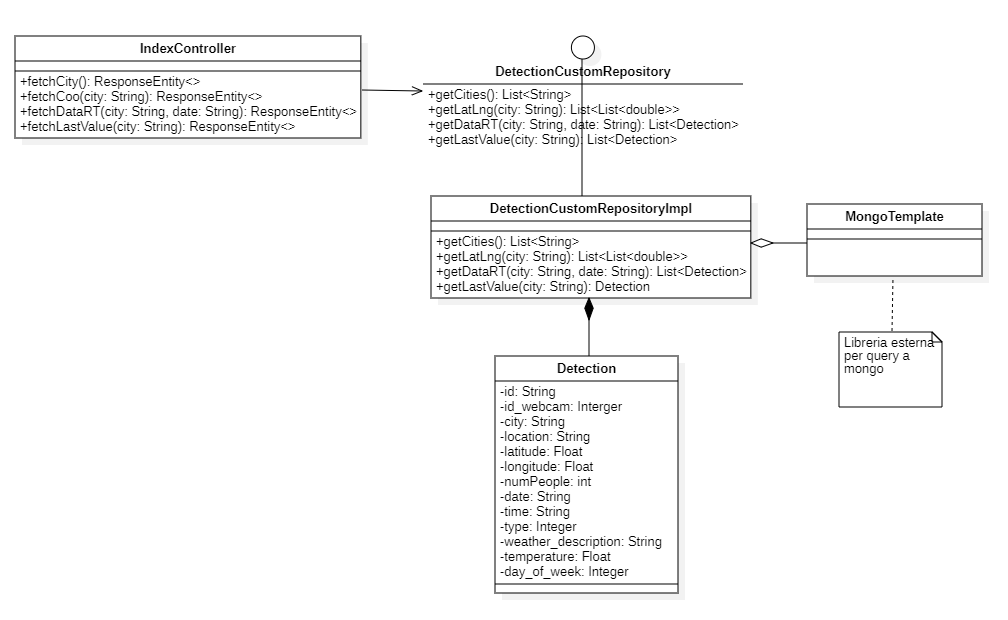
\includegraphics[scale=0.6]{../immagini/diag_PB/diag_class_spring.png}
    \caption{Diagramma delle classi di Spring}
  \end{center}
\end{figure}

\subsection{Diagramma di sequenza}\label{ArchitetturaModuloWebAppDiagrammaDiSequenza}
\begin{figure}[H]
  \begin{center}
    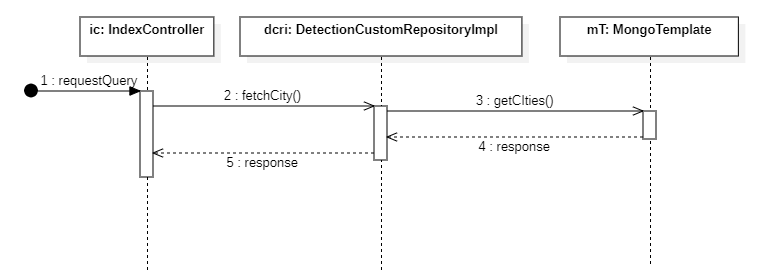
\includegraphics[scale=0.8]{../immagini/diag_PB/diag_seq_spring.png}
    \caption{Diagramma di sequenza di Spring}
  \end{center}
\end{figure}

\subsection{Diagramma di attività}\label{ArchitetturaModuloWebAppDiagrammaDiAttività}
Il diagramma di attività mostrato in seguito descrive la modifica di un parametro attraverso l'interfaccia grafica del prodotto. L'utente all'interno del sito della web-app modifica l'istante di tempo visualizzato dalla mappa, attraverso i componenti dello slider, calendario e la selezione della città. Effettuata questa modifica vengono richiesti al back-end i dati relativi ai parametri inseriti. Il front-end a seguito della ricezione della risposta mostra all'utente la mappa aggiornata con i nuovi dati o un messaggio di errore della mancanza di informazioni per quei parametri inseriti. L'attività arriva al termine a seguito di una di queste due azioni.
\begin{figure}[H]
  \begin{center}
    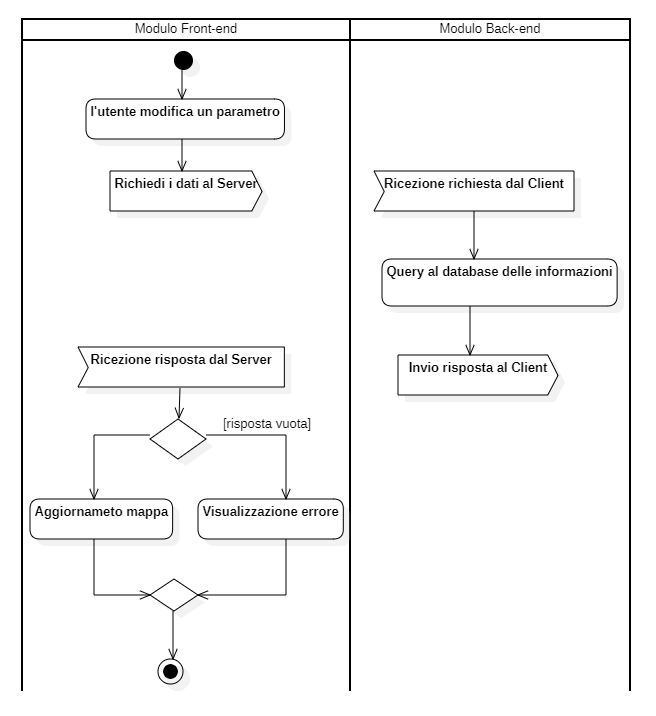
\includegraphics[scale=0.8]{../immagini/diag_PB/diag_act_front_back.png}
    \caption{Diagramma di attività del modulo Web-app}
  \end{center}
\end{figure}
